\documentclass[]{article}
\usepackage[nonatbib]{neurips_2021}
\usepackage[utf8]{inputenc}
\usepackage[T1]{fontenc}
\usepackage{amsfonts}
\usepackage{amsmath}
\usepackage{booktabs}
\usepackage{caption}
\usepackage{color}
\usepackage{courier}
\usepackage{graphicx}
\usepackage{adjustbox}
\usepackage{makecell}
\usepackage{microtype}
\usepackage{multirow,makecell}
\usepackage{nicefrac}
\usepackage{subcaption}
\usepackage{url}
\usepackage{xcolor}
\usepackage{hyperref}
\usepackage{cleveref}
\usepackage{xcolor,colortbl}
\usepackage{pgfplots}
\newif\ifdark
\IfFileExists{/Users/vedaldi/.bash_profile}{
\makeatletter
\immediate\write18{\unexpanded{%
if defaults read -g AppleInterfaceStyle 2>/dev/null;
then echo \\darktrue > /tmp/displaymode.tex;
else echo \\darkfalse > /tmp/displaymode.tex; fi}}
\makeatother 
\input{/tmp/displaymode.tex}
\ifdark
\definecolor{pcolor}{HTML}{1E1E1E}
\definecolor{tcolor}{HTML}{C5C5C5}
\else
\definecolor{pcolor}{HTML}{FDF6E3}
\definecolor{tcolor}{HTML}{333333}
\fi
\pagecolor{pcolor}
\color{tcolor}
% Suppress hbadness warnings.
\hbadness=\maxdimen
\vbadness=\maxdimen
\vfuzz=30pt
\hfuzz=30pt
}{} 
\pgfplotsset{compat=1.17}
\usepackage{caption}
\usepackage{subcaption}

% No space paragraph.
\makeatletter
\renewcommand{\paragraph}{%
  \@startsection{paragraph}{4}%
  %{\z@}{3.25ex \@plus 1ex \@minus .2ex}{-1em}%
  {\z@}{0em}{-1em}%
  {\normalfont\normalsize\bfseries}%
}

\title{Lifting 2D Object Locations to 3D by Discounting LiDAR Outliers across Objects and Views (Supplementary Material)}

\begin{document}

%\maketitle


\section{Additional Results}
In table \ref{t:averageprecision_supp} we provide results for our method with the Mask R-CNN detector trained on the more application-specific Cityscapes\cite{cordts16the-cityscapes} dataset. In particular, running Cityscapes-trained detector on KITTI validation set produces approximately $12000$ detections, whereas COCO-trained detector yields almost $15600$ detections, many of which are of a general vehicle class and not annotated as cars in KITTI. This has advantages at training time, as our network's capacity is not used to attempt fitting non-car objects and also at test time, as we get a lower false positive rate, which results in an overall higher performance.

We also provide additional qualitative examples in figure \ref{f:Qualitative_supp}. In (a,i,l)e of these images we observe cars predicted in green which are not annotated in red, some of this can be attributed to KITTI's particular classification of an object to a non-car vehicle category. In other cases (l) we see cars annotated further away which are annotated in future frames (m), implying issues with KITTI not annotating every car all the time. Two images (c,j) also contain trailers which COCO trained Mask R-CNN detected as cars. KITTI annotates about 3000 examples for each difficulty category with some sequences having annotations frame by frame, some every second frame and other sequences not containing many annotations which may make some detection errors more prominent than others if the number of annotated frames where an object erroneously detected are denser.

\begin{table*}[t]
\newcommand{\zero}{ZERO}
\centering
\setlength{\tabcolsep}{1mm}
\begin{tabular}{cc c c c  c c c}
\toprule
&\multirow{3}{*}{Method} & \multicolumn{3}{c}{Annotations Source} & \multicolumn{3}{c}{AP\textsubscript{BEV}~/~AP\textsubscript{3D} (IoU = 0.5)} \\
&& \textbf{2D} & \multicolumn{2}{c}{\textbf{3D}}  \\
&& Boxes & Yaw & Boxes & Easy & Moderate & Hard \\
\cmidrule(r){1-2}
\cmidrule(lr){3-3}
\cmidrule(lr){4-5}
\cmidrule(l){6-8}

(a) &VS3D~\cite{meng2020ws3d} & Pascal 3D & NYC Cars & & 74.5/40.32 & 66.71/37.36 & 57.55/31.09 \\
\hline
(b) &Zakharov et al. \cite{sdflabel} & KITTI & KITTI &  & 77.84/62.25 & 59.75/42.23 & -/- \\
% Cremers paper here?
% (c) &\textbf{ours} &MS-COCO & &  & \textbf{80.73±2.64}/\textbf{76.73±2.4} & \textbf{81.70±1.29}/\textbf{76.66±1.23} & \textbf{73.61±1.11}/\textbf{69.01±1.03} \\
\hline
(c) &\textbf{ours} &MS-COCO & &  & 80.73/ 76.73 & 81.70/76.66 & 73.61/69.01 \\

% (d) &\textbf{ours} &MS-COCO & KITTI GT &  & & & \\

(e) &\textbf{ours} & Cityscapes & &  & \textbf{86.51}/ \textbf{81.47} & \textbf{84.36}/\textbf{75.49} & \textbf{75.49}/\textbf{68.30} \\

% (f) &\textbf{ours} & Cityscapes & KITTI GT &  & & & \\
% \textbf{86.51}/ \textbf{81.47} & \textbf{84.36}/\textbf{75.49} & \textbf{75.49}/\textbf{68.30} \\

\hline
(g) &\textit{Frus.PointNet~\cite{qi2017frustum} }     & \textit{KITTI} & \textit{KITTI} & \textit{KITTI} & \textit{98.25/98.10} & \textit{94.92/94.31} & \textit{87.14/86.48} \\
\bottomrule
\end{tabular}
\caption{Object Detection Average-Precision on the Kitti validation set. Compared to our Method VS3D\cite{meng2020ws3d} uses a network trained on Pascal 3D and NYC 3D Cars\cite{xiang_wacv14, MatzenICCV13} to determine the object Yaw and 2D box, while while Zakharov\cite{sdflabel} only considers MASK R-CNN detections with an IOU > $50\%$ compared to a ground truth box and uses a synthetic dataset to train a network which estimates orientation. Using Mask R-CNN trained on Cityscapes\cite{cordts16the-cityscapes} instead of the more generic MS-COCO dataset allows us to reduce the number of false positives. }\label{t:averageprecision_supp}
\end{table*}




\begin{figure}
    \centering
    \begin{tabular}{c c}
        
            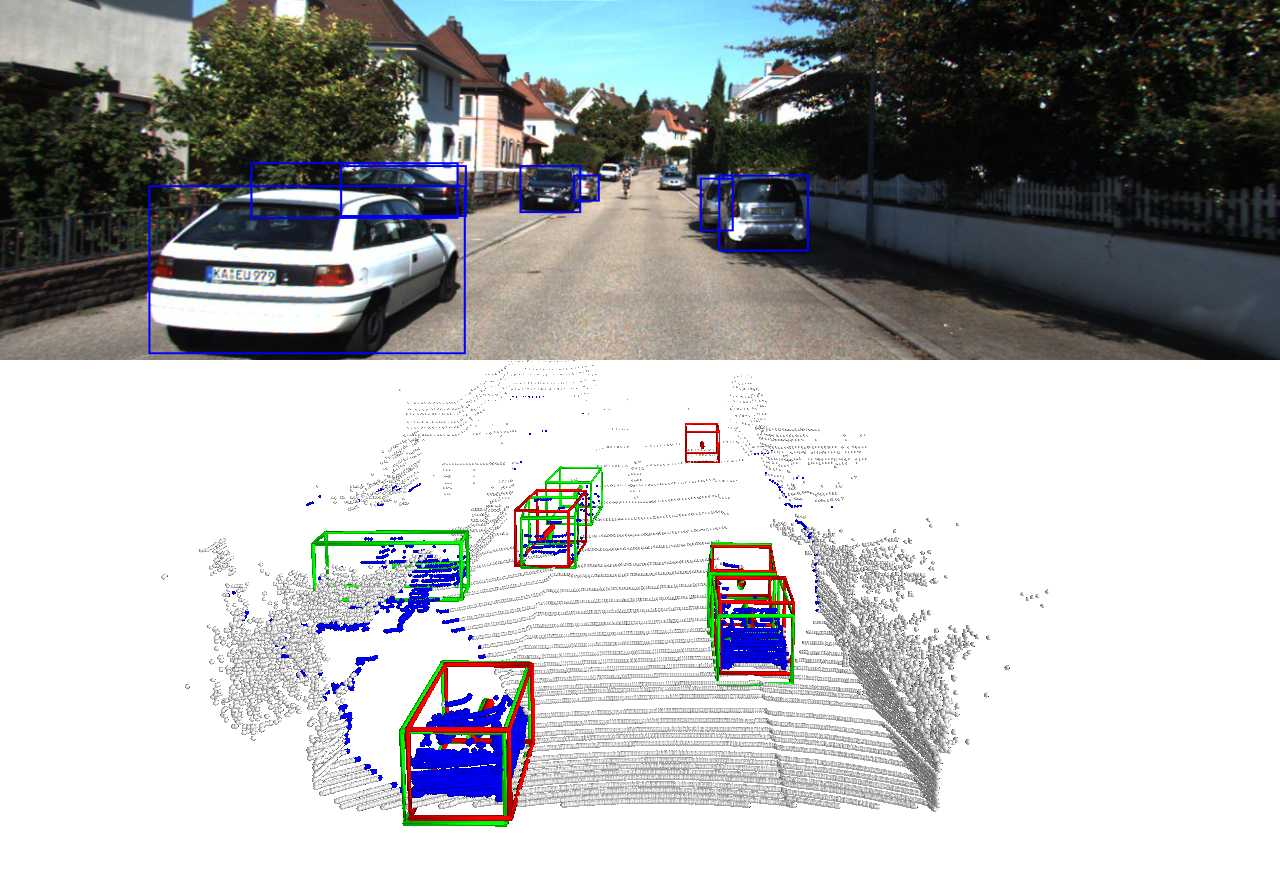
\includegraphics[width=0.5\textwidth]{figures/Qualitative_examples/36.png}
            & 
            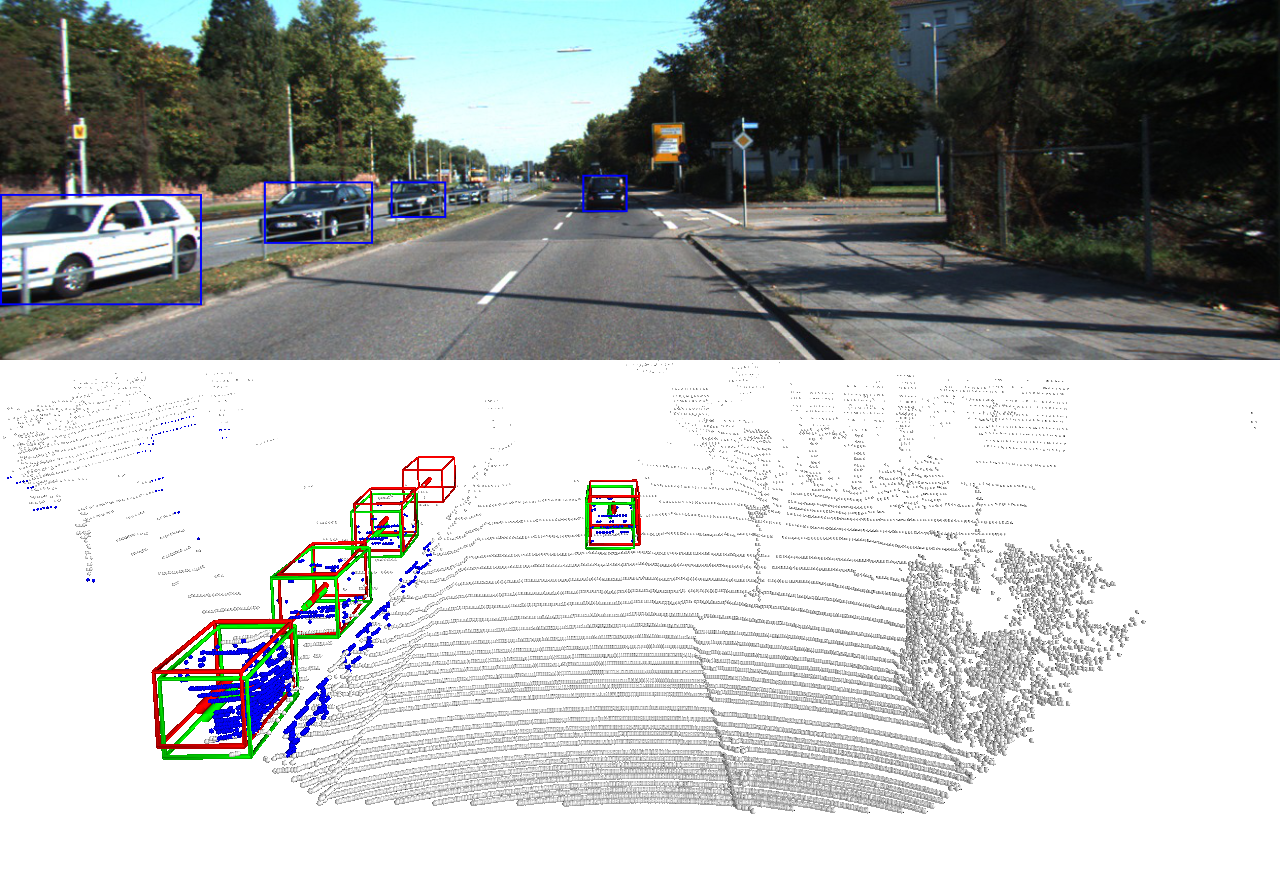
\includegraphics[width=0.5\textwidth]{figures/Qualitative_examples/52.png}
            \\
            a & b\\
            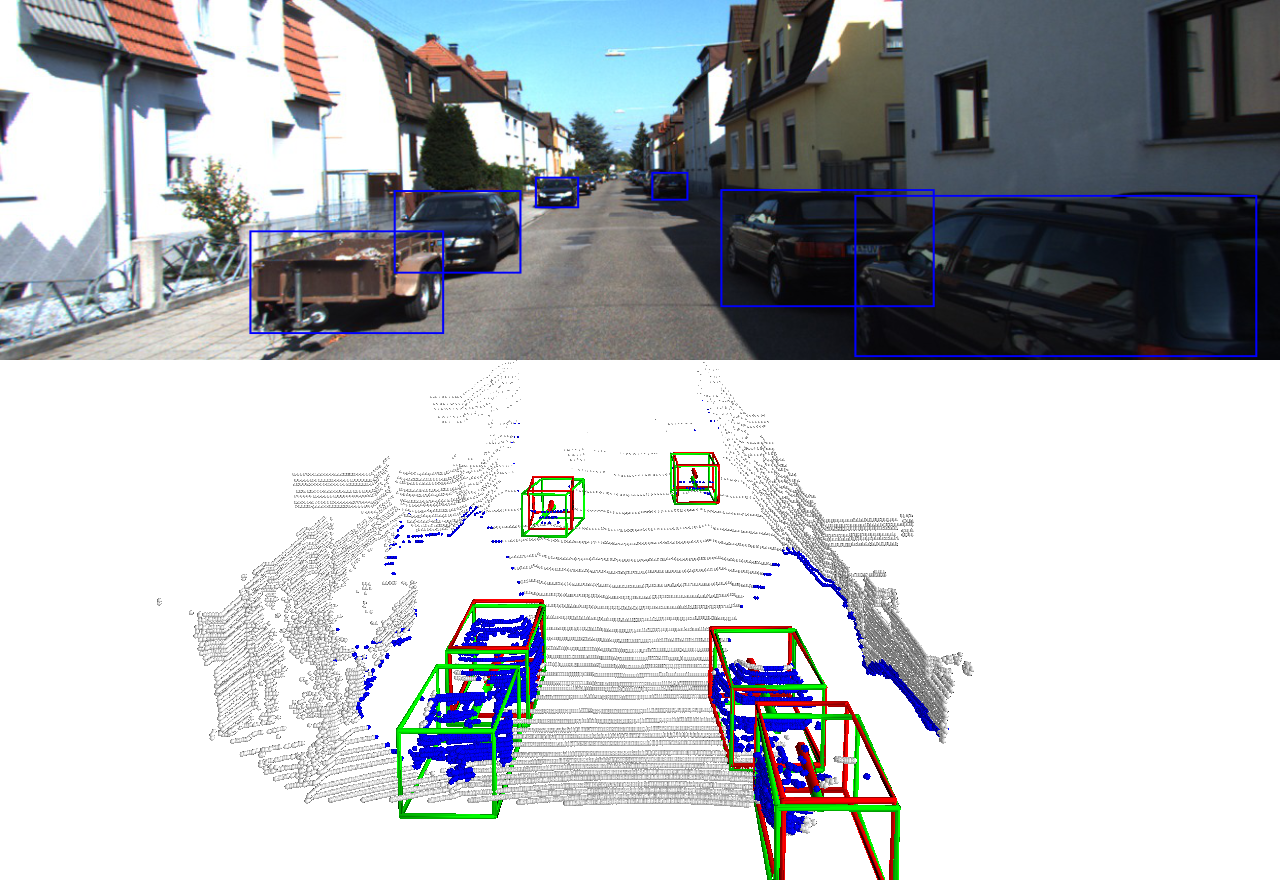
\includegraphics[width=0.5\textwidth]{figures/Qualitative_examples/58.png}
            &  
            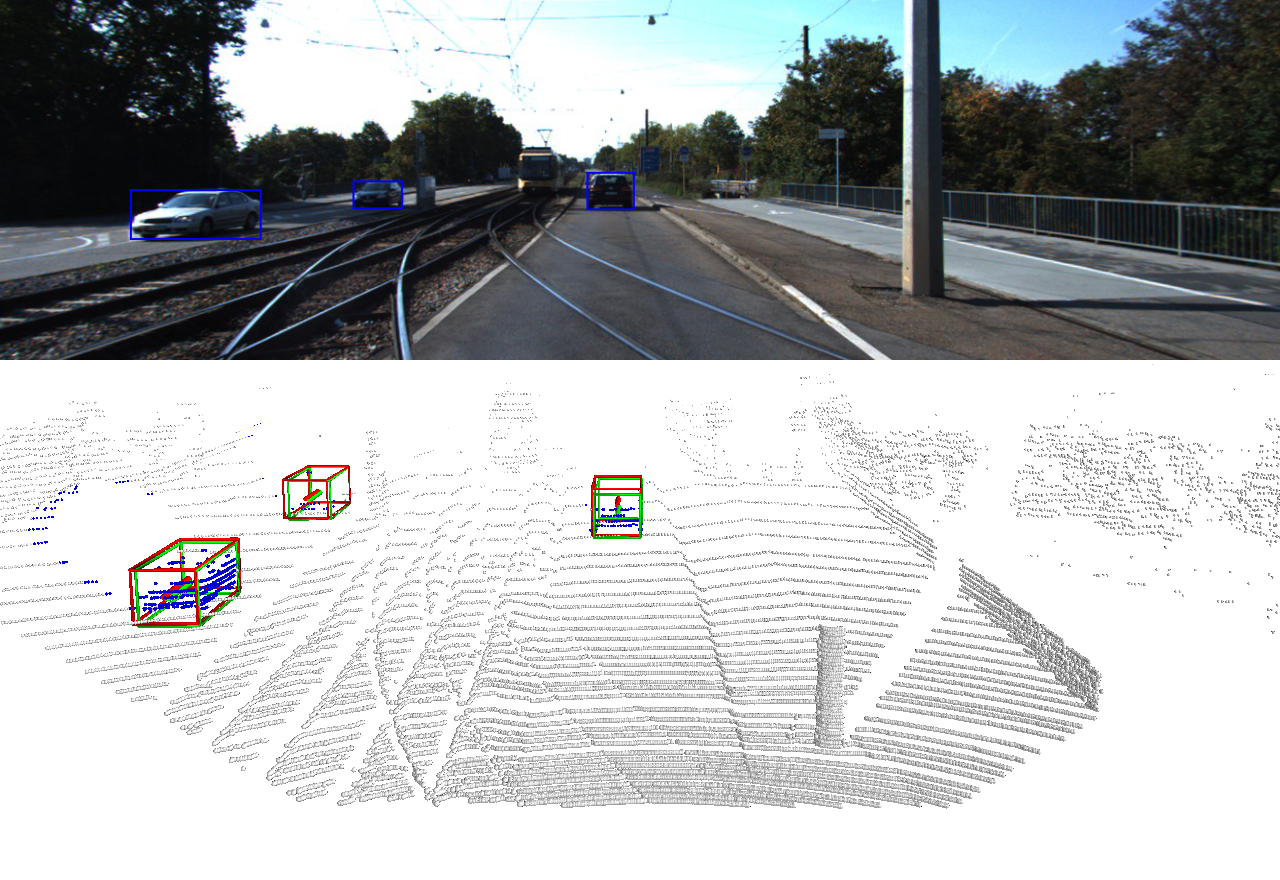
\includegraphics[width=0.5\textwidth]{figures/Qualitative_examples/172.png}
            \\
            c & d\\
        
            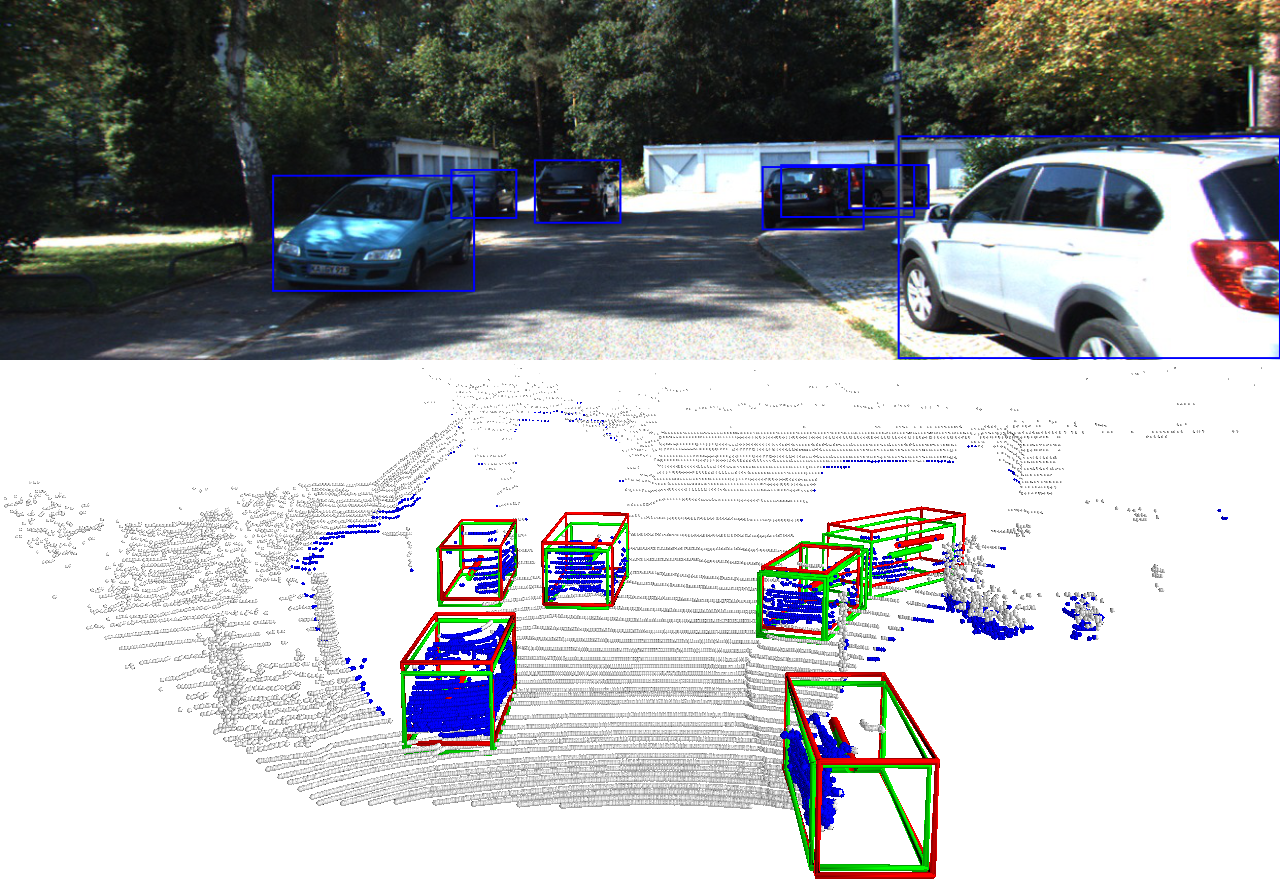
\includegraphics[width=0.5\textwidth]{figures/Qualitative_examples/217.png}
            & 
            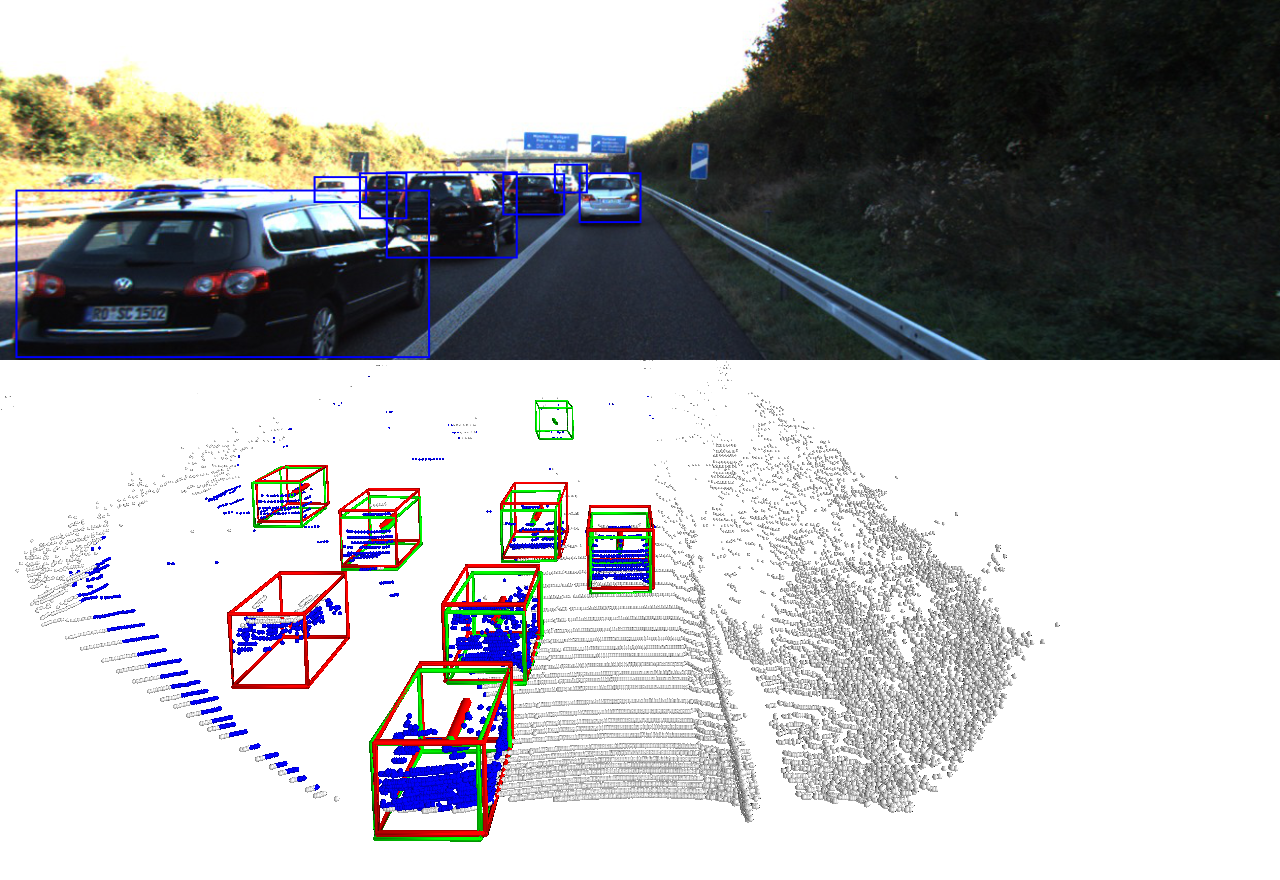
\includegraphics[width=0.5\textwidth]{figures/Qualitative_examples/357.png}
            \\
            e & f\\
        

         
         

 

        
    \end{tabular}
    \caption{Ours in Green, Ground Truth in Red.}
    \label{f:Qualitative_supp}
\end{figure}

\begin{figure}
    \centering
    \begin{tabular}{c c}

        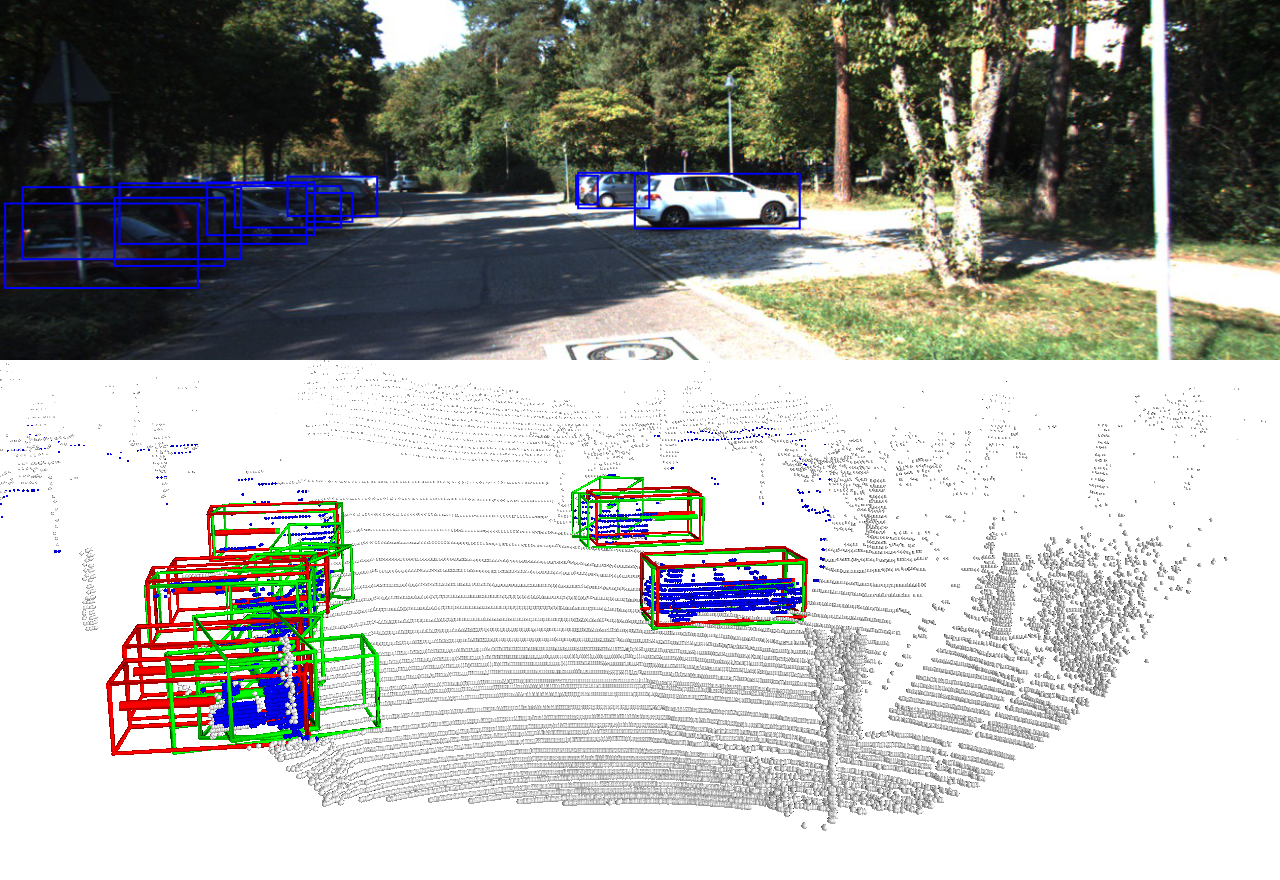
\includegraphics[width=0.5\textwidth]{figures/Qualitative_examples/2.png} &
        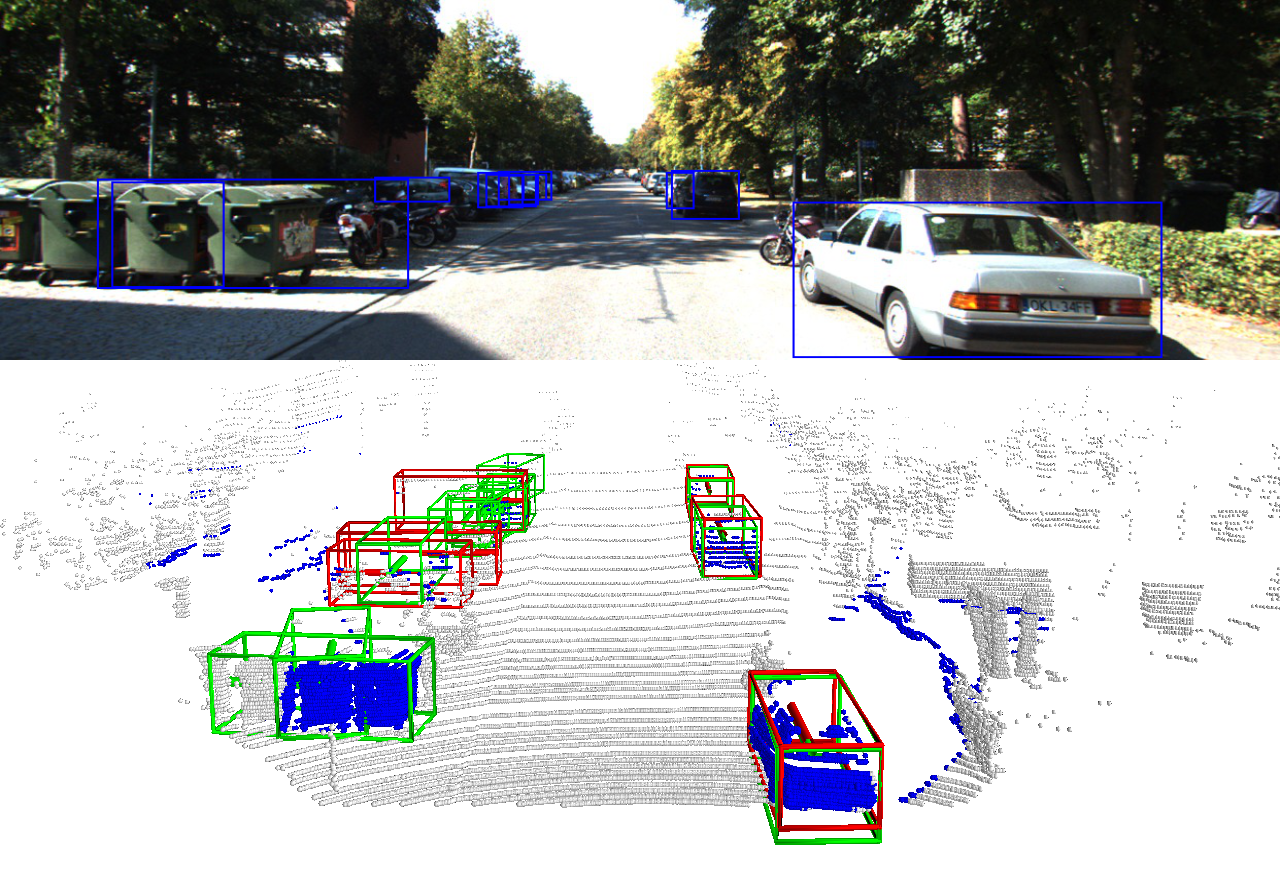
\includegraphics[width=0.5\textwidth]{figures/Qualitative_examples/166.png} \\
        g & h \\ 
        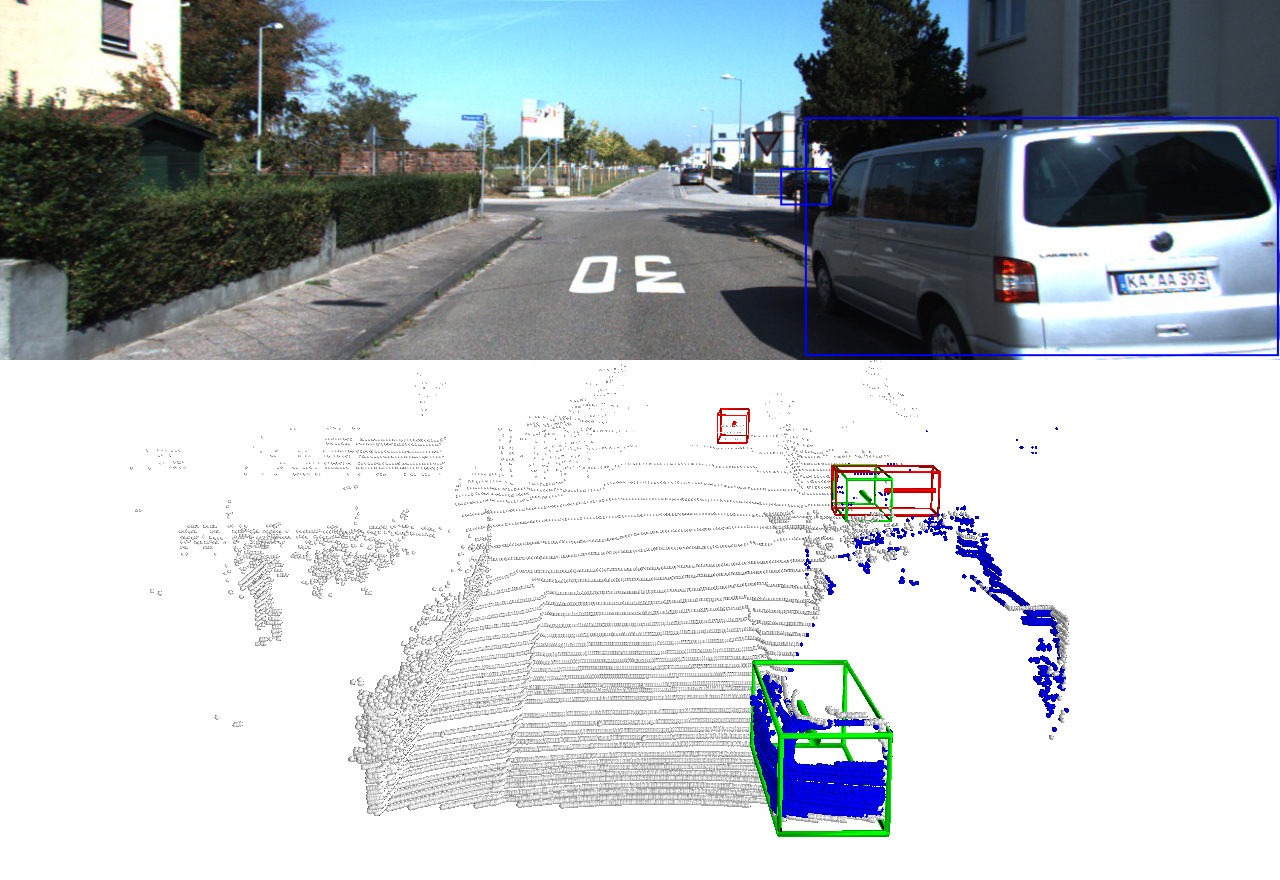
\includegraphics[width=0.5\textwidth]{figures/Qualitative_examples/365.png}
        &
        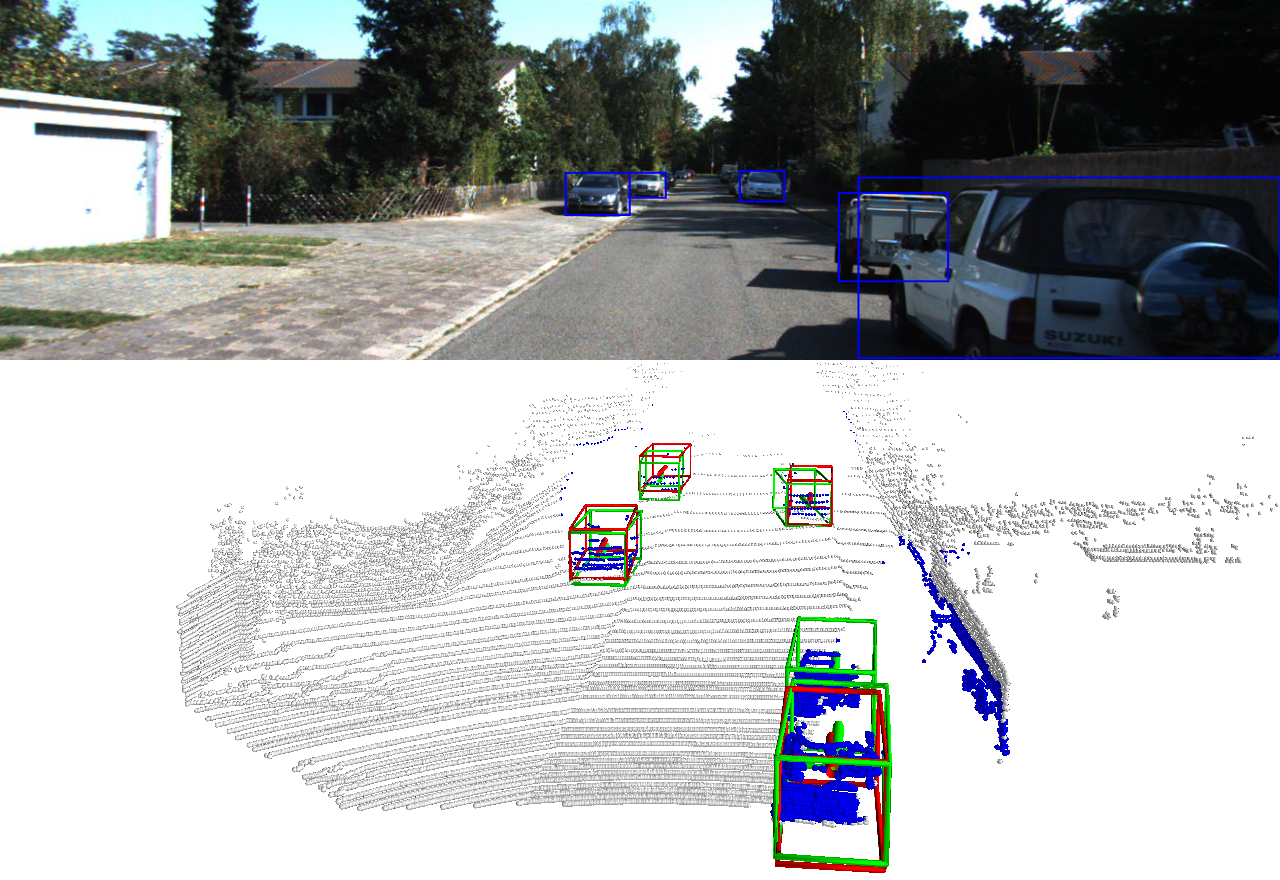
\includegraphics[width=0.5\textwidth]{figures/Qualitative_examples/369.png}
        \\
        i & j \\
         
        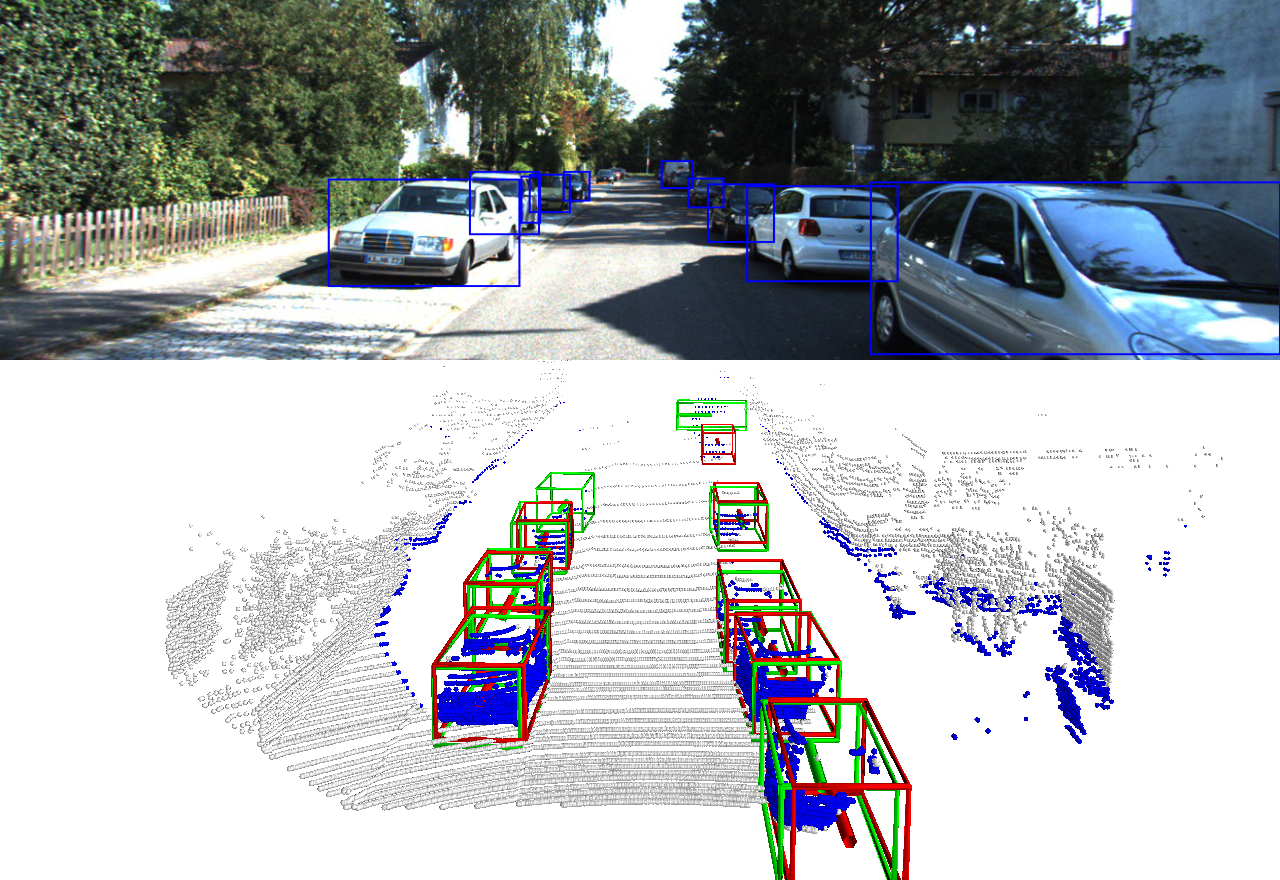
\includegraphics[width=0.5\textwidth]{figures/Qualitative_examples/405.png}
        &
        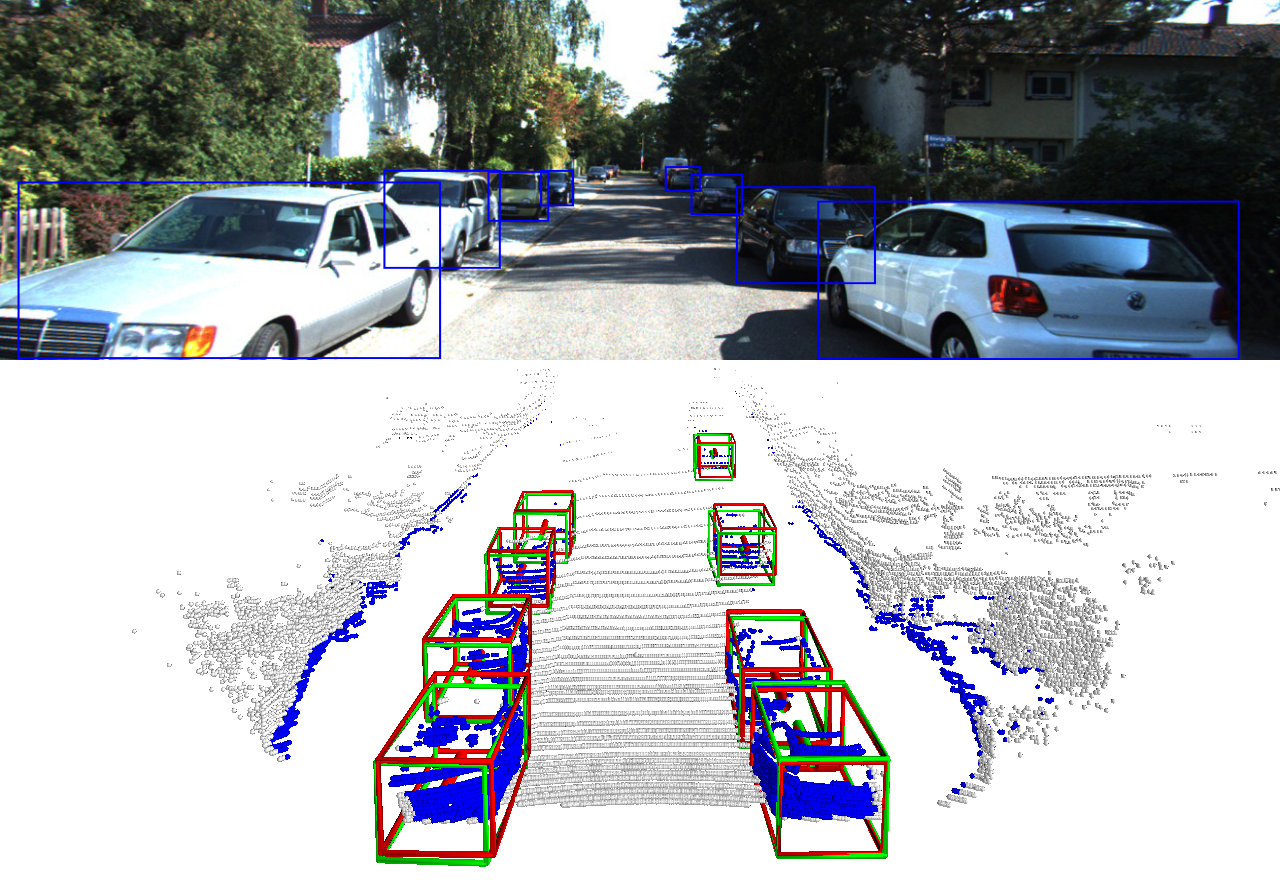
\includegraphics[width=0.5\textwidth]{figures/Qualitative_examples/411.png}
        \\
        l & m \\
% 411,50,314,245
    \end{tabular}
    \caption{Ours in Green, Ground Truth in Red.}
    \label{f:Qualitative_supp2}
\end{figure}


{\small \bibliographystyle{plain}\bibliography{mccraith_g,vedaldi_general,vedaldi_specific, insafutdinov}}

\end{document}